\documentclass[12pt, a4paper]{article}
\usepackage{../../../myconfig} % Gọi file cấu hình từ ngoài gốc vào

% ==========================================
% BẮT ĐẦU NỘI DUNG TÀI LIỆU
% ==========================================
\begin{document}

% Truyền 3 tham số: {Nhãn cam} {Chữ to chính giữa} {Chữ ở góc phải Header}
\titlebox{Chủ đề: định kì}{Đề kiểm tra định kì lần 2}{Đề định kì}

\textit{\textbf{Phần I: Thí sinh trả lời từ câu 1 đến câu 12, mỗi câu thí sinh chỉ chọn một phương án}}

\vspace{0.5cm}

% --- CÂU 1 ---
\questionLinesManual{0}{1}{Cho hàm số \( y = f(x) \) liên tục trên \( \mathbb{R} \) và có đạo hàm  
\(f'(x) = (1-x)^2(x+1)^3(3-x).\) 
Hàm số \( y = f(x) \) đồng biến trên khoảng nào dưới đây?}{%
    \begin{tasks}(4)
        \task \((-\infty; 1)\)
        \task \((-\infty; -1)\)
        \task \((1; 3)\)
        \task \((3; +\infty)\)
    \end{tasks}
}

% --- CÂU 2 ---
\questionLinesManual{0}{2}{Tìm giá trị cực tiểu của hàm số \( y = -x^3 + 3x - 4 \).}{%
    \begin{tasks}(4)
        \task \( -6 \)
        \task \( -1 \)
        \task \( -2 \)
        \task \( 1 \)
    \end{tasks}
}

% --- CÂU 3 ---
\questionLinesManual{0}{3}{Giá trị nhỏ nhất của hàm số \( y = \sqrt{4 - x} + \sqrt{3} \) trên tập xác định của nó là}{%
    \begin{tasks}(4)
        \task \( 2 + \sqrt{3} \)
        \task \( 2\sqrt{3} \)
        \task 0
        \task \( \sqrt{3} \)
    \end{tasks}
}

% --- CÂU 4 ---
\questionLinesManual{0}{4}{Phương trình \( \cos\left(x + \dfrac{\pi}{3}\right) = 1 \) có nghiệm là:}{%
    \begin{tasks}(2)
        \task \( x = -\dfrac{\pi}{3} + k2\pi \, (k \in \mathbb{Z}) \)
        \task \( x = -\dfrac{\pi}{3} + k\pi \, (k \in \mathbb{Z}) \)
        \task \( x = -\dfrac{5\pi}{6} + k2\pi \, (k \in \mathbb{Z}) \)
        \task \( x = \dfrac{\pi}{6} + k2\pi \, (k \in \mathbb{Z}) \)
    \end{tasks}
}


% --- CÂU 5 ---
\questionLinesManual{0}{5}{Cho hàm số \( y = f(x) \). Đồ thị hàm số \( y = f'(x) \) như hình vẽ sau.

\begin{center}
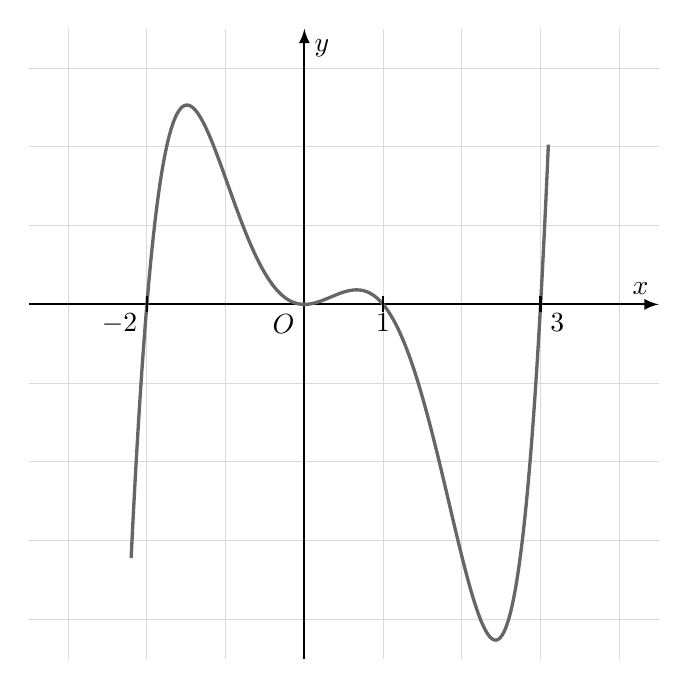
\begin{tikzpicture}[scale=1.0, >=latex]

    % 1. Vẽ lưới tọa độ ô vuông
    \draw[gray!30, thin] (-3.5, -4.5) grid (4.5, 3.5);

    % 2. Trục tọa độ Ox, Oy
    \draw[->, thick] (-3.5, 0) -- (4.5, 0) node[above left] {$x$};
    \draw[->, thick] (0, -4.5) -- (0, 3.5) node[below right] {$y$};

    % Gốc tọa độ O
    \node[below left] at (0, 0) {$O$};

    % 3. Đồ thị hàm số y = f(x)
    % Hàm số đi qua các nghiệm x = -2, x = 0 (kép/tiếp xúc), x = 1, x = 3
    % Công thức đồ thị: y = 0.25 * x^2 * (x + 2) * (x - 1) * (x - 3)
    \draw[very thick, gray!80!black, smooth, domain=-2.2:3.1, samples=200] 
        plot (\x, {0.2*\x*\x*(\x + 2)*(\x - 1)*(\x - 3)});

    % 4. Đánh dấu các vạch chia và nhãn số trên trục Ox
    % x = -2
    \draw[thick] (-2, -0.1) -- (-2, 0.1);
    \node[below left] at (-2, 0) {$-2$};

    % x = 1
    \draw[thick] (1, -0.1) -- (1, 0.1);
    \node[below] at (1, 0) {$1$};

    % x = 3
    \draw[thick] (3, -0.1) -- (3, 0.1);
    \node[below right] at (3, 0) {$3$};

\end{tikzpicture}
\end{center}

Hàm số \( g(x) = f(x) \) có bao nhiêu điểm cực trị?}{%
    \begin{tasks}(4)
        \task 3
        \task 5
        \task 4
        \task 2
    \end{tasks}
}

% --- CÂU 6 ---
\questionLinesManual{0}{6}{Cho hàm số bậc ba \( y = f(x) \) có đồ thị là đường cong trong hình bên.  
Số nghiệm thực của phương trình \( f(x) = 1 \) là

\begin{center}
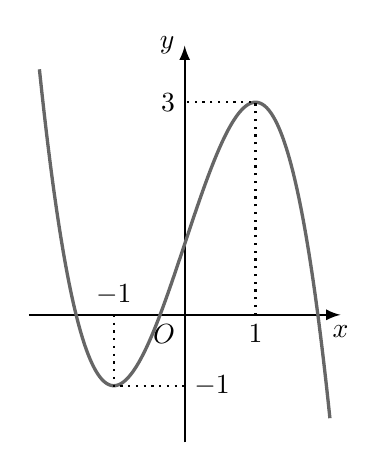
\begin{tikzpicture}[scale=0.9, >=latex]

    % 1. Trục tọa độ Ox, Oy
    \draw[->, thick] (-2.2, 0) -- (2.2, 0) node[below] {$x$};
    \draw[->, thick] (0, -1.8) -- (0, 3.8) node[left] {$y$};

    % Gốc tọa độ O
    \node[below left] at (0, 0) {$O$};

    % 2. Đồ thị hàm số bậc ba y = f(x) = -x^3 + 3x + 1
    % Cực tiểu tại (-1, -1) và Cực đại tại (1, 3)
    \draw[very thick, gray!80!black, smooth, domain=-2.05:2.05, samples=200] 
        plot (\x, {-\x*\x*\x + 3*\x + 1});

    % 3. Đường nét đứt gióng các cực trị
    % Cực tiểu (-1, -1)
    \draw[dotted, thick, black] (-1, 0) -- (-1, -1) -- (0, -1);
    
    % Cực đại (1, 3)
    \draw[dotted, thick, black] (1, 0) -- (1, 3) -- (0, 3);

    % 4. Đánh dấu các giá trị trên trục
    \node[above] at (-1, 0) {$-1$};
    \node[below] at (1, 0) {$1$};
    \node[right] at (0, -1) {$-1$};
    \node[left] at (0, 3) {$3$};

\end{tikzpicture}
\end{center}
}{%
    \begin{tasks}(4)
        \task 0
        \task 3
        \task 1
        \task 2
    \end{tasks}
}

% --- CÂU 7 ---
\questionLinesManual{0}{7}{Cho cấp số cộng \( (u_n) \) biết \( u_1 = 2 \), công sai \( d = -5 \). Tổng 10 số hạng đầu của cấp số cộng đó là}{%
    \begin{tasks}(4)
        \task \(-410\)
        \task \(-205\)
        \task \(245\)
        \task \(-230\)
    \end{tasks}
}

% --- CÂU 8 ---
\questionLinesManual{0}{8}{Cho hàm số \( f(x) \) xác định trên \( \mathbb{R} \setminus \left\{ \dfrac{1}{2} \right\} \) thỏa mãn
\( f'(x) = \dfrac{2}{2x-1}\), \( f(0) = 1, \, f(1) = 2. \)
Giá trị của biểu thức \( f(-1) + f(3) \) bằng}{%
    \begin{tasks}(4)
        \task \( 2 + \ln 15 \)
        \task \( 3 + \ln 15 \)
        \task \( \ln 15 \)
        \task \( 4 + \ln 15 \)
    \end{tasks}
}

% --- CÂU 9 ---
\questionLinesManual{0}{9}{Tìm số tiệm cận đứng của đồ thị hàm số:  
\(y = \dfrac{x^2 - 3x - 4}{x^2 - 16}\)}{%
    \begin{tasks}(4)
        \task 2
        \task 3
        \task 1
        \task 0
    \end{tasks}
}

% --- CÂU 10 ---
\questionLinesManual{0}{10}{Cho hàm số \( y = \dfrac{ax + b}{cx + d} \) có đồ thị như sau.

\begin{center}
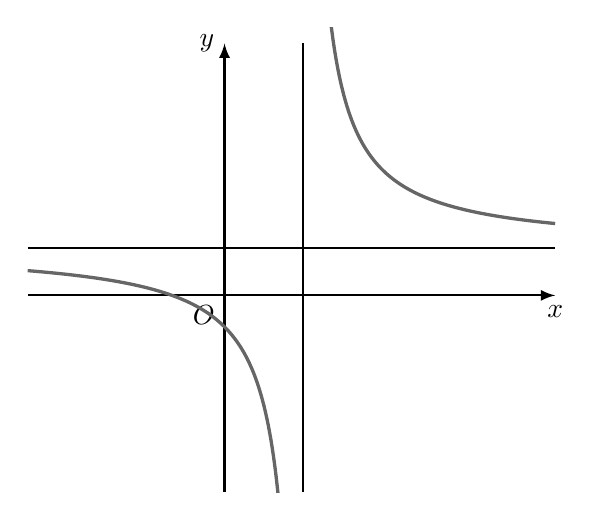
\begin{tikzpicture}[scale=1.0, >=latex]
    \clip (-2.5, -2.5) rectangle (4.4, 3.4);
    % 1. Trục tọa độ Ox, Oy
    \draw[->, thick] (-2.5, 0) -- (4.2, 0) node[below] {$x$};
    \draw[->, thick] (0, -2.5) -- (0, 3.2) node[left] {$y$};

    % Gốc tọa độ O
    \node[below left] at (0, 0) {$O$};

    % 2. Các đường tiệm cận
    % Tiệm cận đứng x = 1 (x = -d/c > 0)
    \draw[thick] (1, -2.5) -- (1, 3.2);

    % Tiệm cận ngang y = 0.6 (y = a/c > 0)
    \draw[thick] (-2.5, 0.6) -- (4.2, 0.6);

    % 3. Hai nhánh của đồ thị hàm số y = (0.6x - 0.4)/(x - 1)
    % Cắt Oy tại y = -0.4 (< 0), cắt Ox tại x ≈ 0.67 (> 0 nhưng < 1)
    
    % Nhánh bên trái tiệm cận đứng (x < 1)
    \draw[very thick, gray!80!black, smooth, domain=-2.5:0.75, samples=100] 
        plot (\x, {(0.6*\x + 0.4)/(\x - 1)});

    % Nhánh bên phải tiệm cận đứng (x > 1)
    \draw[very thick, gray!80!black, smooth, domain=1.35:4.2, samples=100] 
        plot (\x, {(0.6*\x + 0.4)/(\x - 1)});

\end{tikzpicture}
\end{center}

Mệnh đề nào sau đây đúng?}{%
    \begin{tasks}(2)
        \task \( ac > 0; \, bd > 0 \)
        \task \( ab < 0; \, cd < 0 \)
        \task \( bc > 0; \, ad < 0 \)
        \task \( ad > 0; \, bd < 0 \)
    \end{tasks}
}

% --- CÂU 11 ---
\questionLinesManual{0}{11}{Biểu thức \( T = \sqrt[5]{a^3} \) với \( a > 0 \), được viết dưới dạng luỹ thừa với số mũ hữu tỉ là}{%
    \begin{tasks}(4)
        \task \( a^{\frac{3}{5}} \)
        \task \( a^{\frac{2}{15}} \)
        \task \( a^{\frac{4}{15}} \)
        \task \( a^{\frac{3}{10}} \)
    \end{tasks}
}

% --- CÂU 12 ---
\questionLinesManual{0}{12}{Biết \( \displaystyle\int_{0}^{1} [f(x) + 2x] dx = 3 \). Khi đó \( \displaystyle\int_{0}^{1} f(x) dx \) bằng}{%
    \begin{tasks}(4)
        \task 1
        \task 5
        \task 3
        \task 2
    \end{tasks}
}

\textit{\textbf{Phần II: Thí sinh trả lời từ câu 13 đến câu 16; trong mỗi ý a), b), c), d) ở mỗi câu, thí sinh chọn đúng hoặc sai.}}

\vspace{0.3cm}

%Câu 30 trong 35 chuyên đè phân dúng sai UDTP
\questionTrueFalse{0}{13}{Một công ty thiết kế mẫu huy hiệu để tặng cho khách hàng thân thiết của mình (xem hình vẽ bên dưới). Trong đó \(ABCD\) là hình vuông có cạnh bằng \(4cm\), các đường cong \(AOD\) và \(BOC\) là một phần của các parabol đỉnh \(O\). Với hệ trục tọa độ \(Oxy\) (đơn vị trên mỗi trục tọa độ là cm), thì điểm A có tung độ bằng 1. Biết phần tô đậm trong hình vẽ được phủ vàng với chi phí 1 triệu đồng/\(1cm^2\), phần còn lại được phủ bạc với chi phí 300 nghìn đồng/cm², các chi phí còn lại là 500 nghìn đồng.

\begin{center}
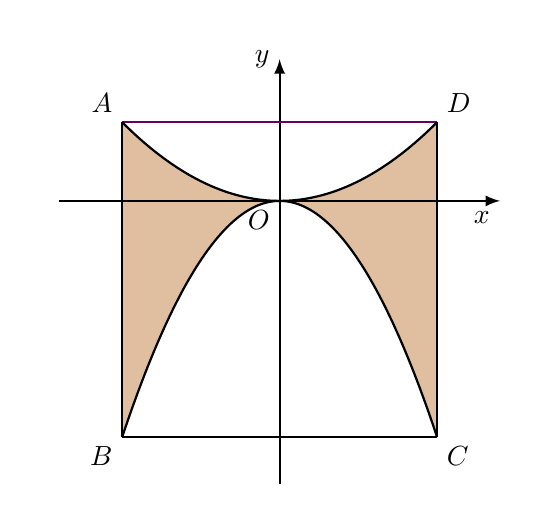
\begin{tikzpicture}[scale=1.0, >=latex]
    % Giới hạn vùng hiển thị bằng lệnh \clip
    \clip (-3.2, -3.8) rectangle (3.2, 2.2);
    % Phần dưới (giữa y = 0.25*x^2 và y = -0.75*x^2)
    \fill[brown!50] plot[domain=-2:2, samples=100] (\x, {0.25*\x*\x}) 
        -- plot[domain=2:-2, samples=100] (\x, {-0.75*\x*\x}) -- cycle;

    % 2. Hệ trục tọa độ Oxy
    \draw[->, thick] (-2.8, 0) -- (2.8, 0) node[below left] {$x$};
    \draw[->, thick] (0, -3.6) -- (0, 1.8) node[left] {$y$};
    \node[below left] at (0, 0) {$O$};

    % 3. Khung hình vuông ABCD
    % A(-2, 1), D(2, 1), B(-2, -3), C(2, -3)
    \draw[thick, violet!80!black] (-2, 1) -- (2, 1); % Cạnh AD
    \draw[thick, black] (-2, -3) -- (2, -3);         % Cạnh BC
    \draw[thick, black] (-2, 1) -- (-2, -3);         % Cạnh AB
    \draw[thick, black] (2, 1) -- (2, -3);           % Cạnh CD

    % 4. Hai đường cong Parabol
    % Parabol AOD: y = 0.25 * x^2
    \draw[thick, black, domain=-2:2, samples=100] plot (\x, {0.25*\x*\x});

    % Parabol BOC: y = -0.75 * x^2
    \draw[thick, black, domain=-2:2, samples=100] plot (\x, {-0.75*\x*\x});

    % 5. Đánh dấu tên các đỉnh A, B, C, D
    \node[above left] at (-2, 1) {$A$};
    \node[above right] at (2, 1) {$D$};
    \node[below left] at (-2, -3) {$B$};
    \node[below right] at (2, -3) {$C$};
\end{tikzpicture}
\end{center}
}{
    \textbf{a)} & Parabol chứa đường cong \(AOD\) có phương trình là  
    \(y = \dfrac{1}{16}x^2\).
    & \textcolor{amberorange}{$\bigcirc$} & \textcolor{amberorange}{$\bigcirc$} \\ \hline
    
    \textbf{b)} & Parabol chứa đường cong \(BOC\) có phương trình là  
    \(y = -\dfrac{3}{4}x^2\).
    & \textcolor{amberorange}{$\bigcirc$} & \textcolor{amberorange}{$\bigcirc$} \\ \hline
    
    \textbf{c)} & Diện tích phần tô đậm trong hình vẽ lớn hơn \(5,5cm^2\).
    & \textcolor{amberorange}{$\bigcirc$} & \textcolor{amberorange}{$\bigcirc$} \\ \hline
    
    \textbf{d)} & Chi phí sản xuất 1 chiếc huy hiệu trên nhỏ hơn 9 triệu đồng.
    & \textcolor{amberorange}{$\bigcirc$} & \textcolor{amberorange}{$\bigcirc$} \\
}

\questionTrueFalse{0}{14}{Nhà máy \( A \) chuyên sản xuất một loại sản phẩm cho nhà máy \( B \). Hai nhà máy thỏa thuận rằng, hằng tháng nhà máy \( A \) cung cấp cho nhà máy \( B \) số lượng sản phẩm theo đơn đặt hàng của nhà máy \( B \). Nếu số lượng đặt hàng là \( x \) tấn sản phẩm thì giá bán mỗi tấn sản phẩm là  
\(P(x) = 45 - 0,001x^2\) (triệu đồng). Chi phí để nhà máy \( A \) sản xuất \( x \) tấn sản phẩm trong một tháng là  
\(C(x) = 100 + 30x\) (triệu đồng).}{
    \textbf{a)} & Chi phí để nhà máy \( A \) sản xuất 10 tấn sản phẩm trong một tháng là 400 triệu đồng.
    & \textcolor{amberorange}{$\bigcirc$} & \textcolor{amberorange}{$\bigcirc$} \\ \hline
    
    \textbf{b)} & Số tiền nhà máy \( A \) thu được khi bán 10 tấn sản phẩm cho nhà máy \( B \) là 600 triệu đồng.
    & \textcolor{amberorange}{$\bigcirc$} & \textcolor{amberorange}{$\bigcirc$} \\ \hline
    
    \textbf{c)} & Lợi nhuận mà nhà máy \( A \) thu được khi bán \( x \) tấn sản phẩm (\( 0 \leq x \leq 100 \)) cho nhà máy \( B \) là  
    \(H(x) = -0,001x^3 + 15x - 100\) (triệu đồng).
    & \textcolor{amberorange}{$\bigcirc$} & \textcolor{amberorange}{$\bigcirc$} \\ \hline
    
    \textbf{d)} & Để thu được lợi nhuận lớn nhất thì mỗi tháng nhà máy \( A \) bán cho nhà máy \( B \) khoảng 70,7 tấn sản phẩm (số tấn làm tròn đến hàng phần chục).
    & \textcolor{amberorange}{$\bigcirc$} & \textcolor{amberorange}{$\bigcirc$} \\
}

\questionTrueFalse{0}{15}{Những ngày giáp Tết Nguyên Đán cũng là dịp bước vào vụ Đông Xuân, bà con nông dân tích cực xuống đồng cấy lúa. Cây lúa sau khi được cấy trải qua quá trình tăng trưởng để nhanh và phát triển chiều cao trước khi làm đòng, trổ bông. Qua nghiên cứu một giống lúa mới, các nhà khoa học nhận thấy một cây lúa tính từ lúc được cấy bằng một cây mạ với chiều cao 20cm có tốc độ tăng trưởng chiều cao cho bởi hàm số \( v(t) = -0,1t^3 + 1,1t^2 \), trong đó \( t \) tính theo tuần, \( v(t) \) tính bằng cm/tuần. Gọi \( h(t) \) là chiều cao của cây lúa ở tuần thứ \( t \) (\( t \geq 0 \)).
\begin{figure}[H]
    \centering
    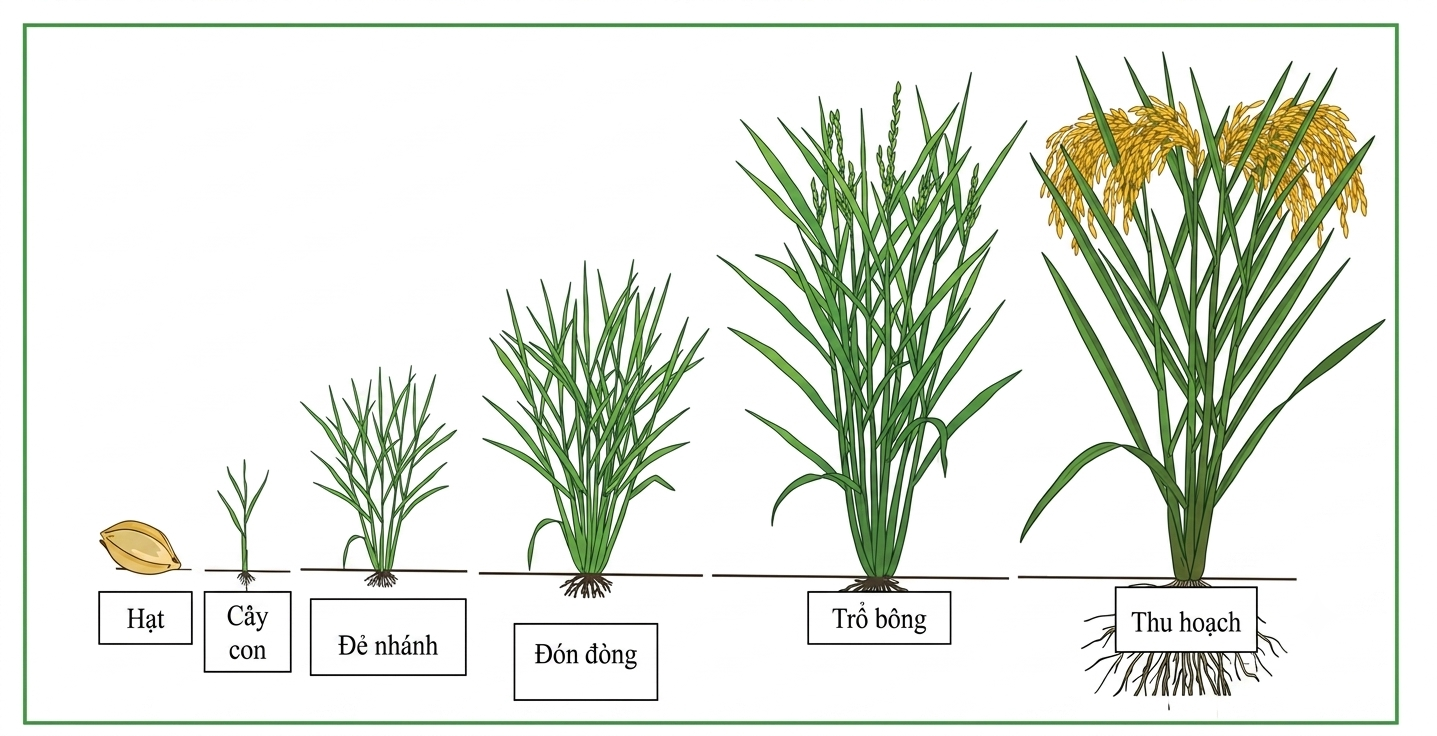
\includegraphics[width=0.4\textwidth]{images/Lua.png}
\end{figure}
}{
    \textbf{a)} & \(h(t) = -\dfrac{1}{40}t^4 + \dfrac{11}{30}t^3 + 20.\)
    & \textcolor{amberorange}{$\bigcirc$} & \textcolor{amberorange}{$\bigcirc$} \\ \hline
    
    \textbf{b)} & Giai đoạn tăng trưởng chiều cao của cây lúa kéo dài 12 tuần.
    & \textcolor{amberorange}{$\bigcirc$} & \textcolor{amberorange}{$\bigcirc$} \\ \hline
    
    \textbf{c)} & Chiều cao tối đa của cây lúa là 150cm.
    & \textcolor{amberorange}{$\bigcirc$} & \textcolor{amberorange}{$\bigcirc$} \\ \hline
    
    \textbf{d)} & Vào thời điểm cây lúa phát triển nhanh nhất, chiều cao của cây đã lớn hơn 80cm.
    & \textcolor{amberorange}{$\bigcirc$} & \textcolor{amberorange}{$\bigcirc$} \\
}



\questionTrueFalse{0}{16}{Một nhà sản xuất muốn thiết kế một hộp đựng kẹo dạng hình tròn xoay gồm hai phần: Phần thứ nhất được tạo thành khi quay "nửa" hình elip quanh một trục; phần thứ hai là nửa hình cầu có bán kính bằng 4 cm. Nếu xét trong hệ trục tọa độ Oxy, đơn vị trên trục là cm thì  
"nửa" hình elip quay quanh trục Ox để tạo thành phần thứ nhất có phương trình là  
\(\dfrac{x^2}{64} + \dfrac{y^2}{16} = 1\)  
với \(-8 \leq x \leq 0\) (xem hình minh họa).
\begin{figure}[H]
    \centering
    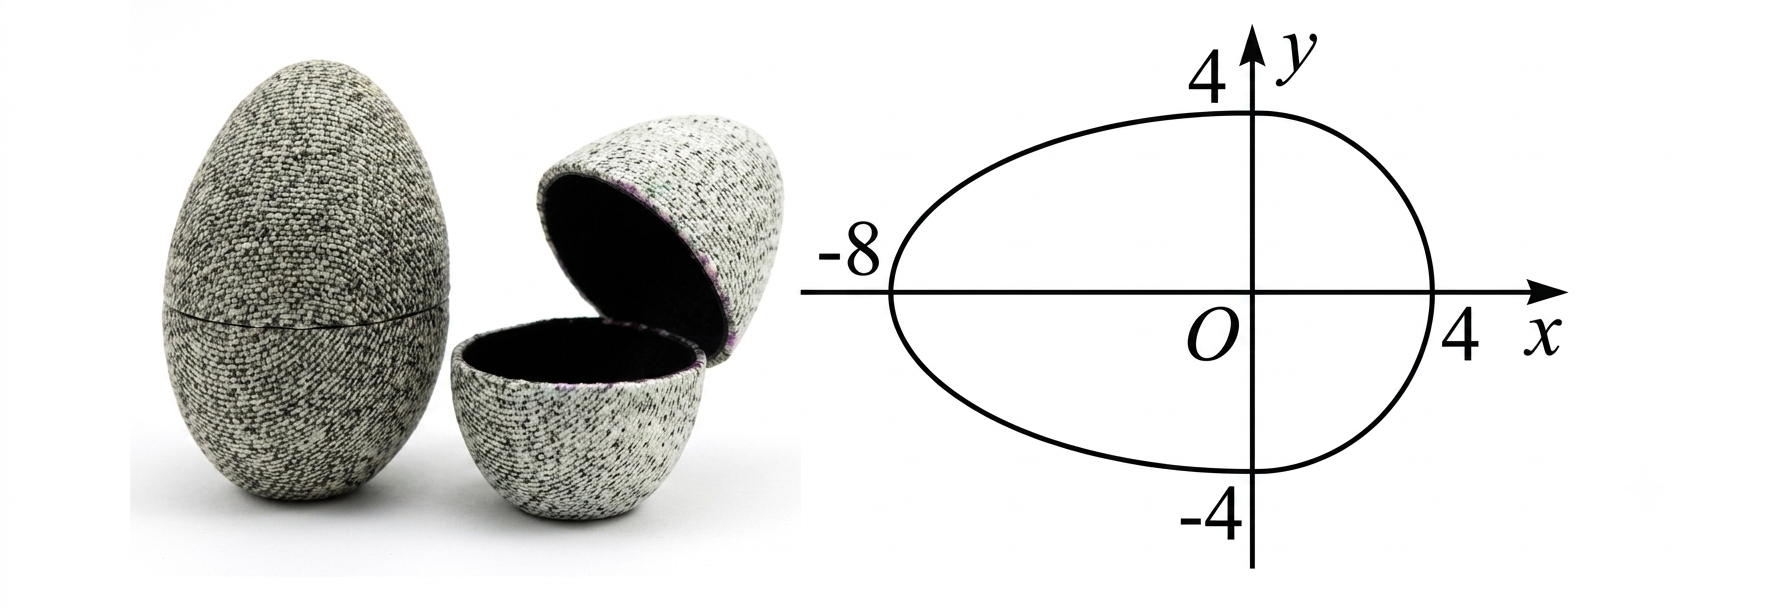
\includegraphics[width=0.5\textwidth]{images/Trung.png}
\end{figure}

}{
    \textbf{a)} & Thể tích của phần không gian "chứa" trong phần thứ hai (nửa khối cầu) bằng  
    \(\dfrac{32}{3} \pi \, (\text{cm}^3)\).
    & \textcolor{amberorange}{$\bigcirc$} & \textcolor{amberorange}{$\bigcirc$} \\ \hline
    
    \textbf{b)} & Đường thuộc góc phần tư thứ hai trong hệ trục Oxy là đồ thị của hàm số  
    \(y = \sqrt{16 - \dfrac{x^2}{4}}, \, -8 \leq x \leq 0.\)
    & \textcolor{amberorange}{$\bigcirc$} & \textcolor{amberorange}{$\bigcirc$} \\ \hline
    
    \textbf{c)} & Thể tích của phần không gian "chứa" trong phần thứ nhất được tính bởi công thức  
    \(V = \pi \displaystyle\int_{-8}^{0} \sqrt{16 - \dfrac{x^2}{4}} \, dx \, (\text{cm}^3).\)
    & \textcolor{amberorange}{$\bigcirc$} & \textcolor{amberorange}{$\bigcirc$} \\ \hline
    
    \textbf{d)} & Thể tích phần không gian bên trong của hộp đựng kẹo cần thiết kế là \(24\pi \, (\text{cm}^3)\).
    & \textcolor{amberorange}{$\bigcirc$} & \textcolor{amberorange}{$\bigcirc$} \\
}

\newpage
\textit{\textbf{Phần III: Thí sinh trả lời từ câu 17 đến câu 22.}}

\vspace{0.3cm}

\questionShortAnswer{0}{17}{Để tích trữ nước ngọt sinh hoạt chuẩn bị cho mùa hạn mặn ở Đồng bằng sông Cửu Long, một hộ dân muốn xây một bể nước không nắp dạng khối hộp chữ nhật không nắp có thể tích bằng \( 200 \, m^3 \). Đáy bể là hình hộp chữ nhật có chiều dài gấp đôi chiều rộng. Biết chi phí xây bể là 850 nghìn đồng/m\(^2\). Hãy tính chi phí thấp nhất mà hộ gia đình cần bỏ ra để xây dựng bể chứa nước ngọt dự trữ (làm tròn đến đơn vị triệu đồng).
\begin{figure}[H]
    \centering
    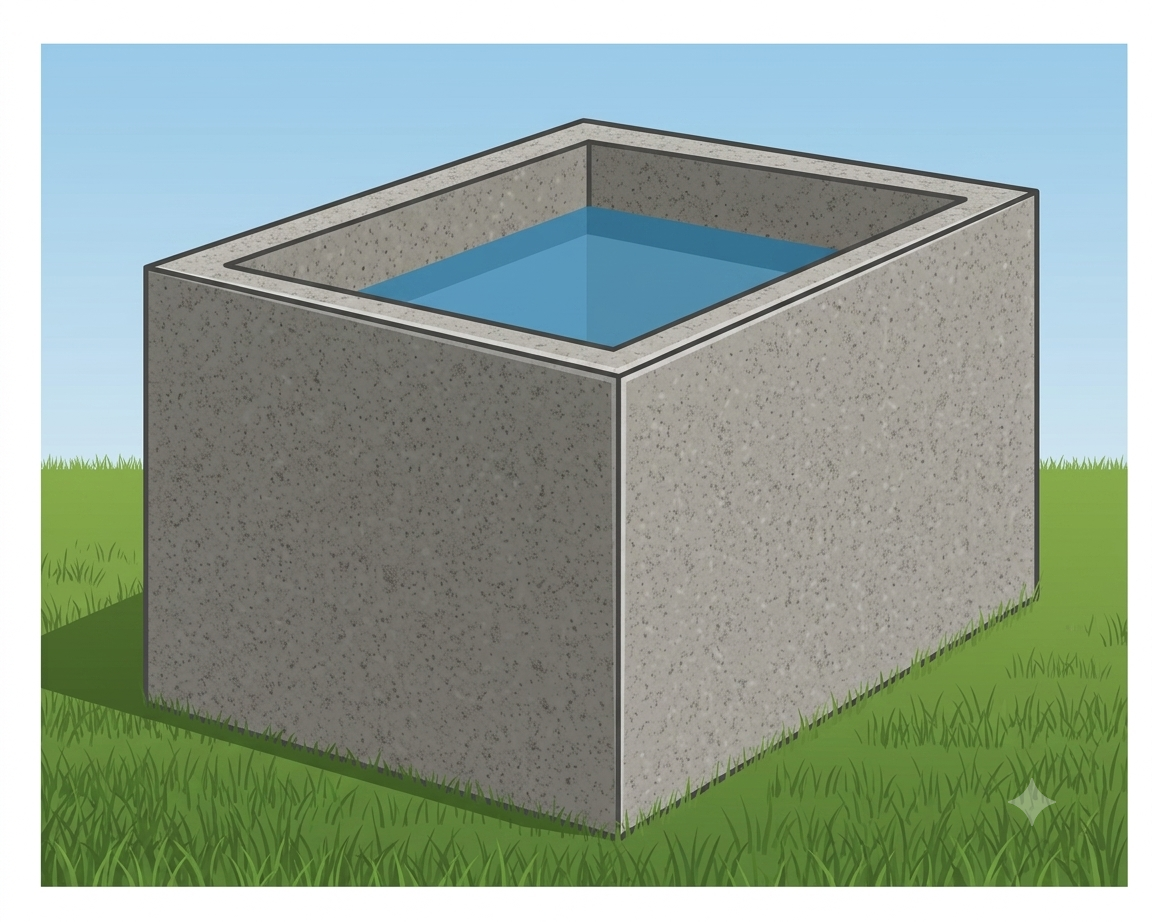
\includegraphics[width=0.3\textwidth]{images/BeNuoc.png}
\end{figure}

}

\questionShortAnswer{0}{18}{Nhà bác Ba có tất cả 8 cánh cửa sắt hình chữ nhật với chiều dài \( 2m \) và chiều rộng \( 1m \). Hai mặt của mỗi cánh cửa được thiết kế như hình vẽ dưới đây. Trong đó, phần được tô đậm được sơn màu xanh, phần còn lại được sơn màu trắng. Mỗi phần sơn màu trắng có đường biên cong là một phần của parabol có đỉnh nằm trên cạnh của hình chữ nhật. Biết rằng chi phí để sơn màu xanh là \( 120 \, \text{nghìn đồng/m}^2 \) và chi phí sơn màu trắng là \( 110 \, \text{nghìn đồng/m}^2 \). Hỏi, để sơn toàn bộ số cửa sắt trên, bác Ba phải tốn bao nhiêu triệu đồng (làm tròn kết quả đến hàng phần trăm theo đơn vị triệu đồng).

\begin{center}
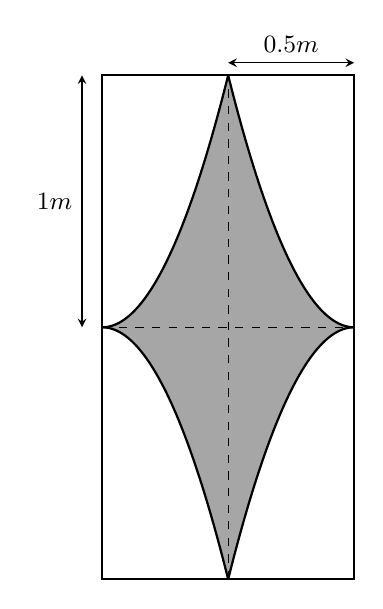
\begin{tikzpicture}[scale=3.2, >=latex]
    % 1. Vẽ khung hình chữ nhật 1m x 2m
    \draw[thick, black] (-0.5, -1) rectangle (0.5, 1);

    % 2. Tô màu xám/xanh cho phần hình bốn cánh ở giữa (sơn xanh)
    \fill[gray!70] 
        plot[domain=0:0.5, samples=50] (\x, {4*(\x-0.5)*(\x-0.5)}) -- 
        plot[domain=0.5:0, samples=50] (\x, {-4*(\x-0.5)*(\x-0.5)}) -- 
        plot[domain=0:-0.5, samples=50] (\x, {-4*(\x+0.5)*(\x+0.5)}) -- 
        plot[domain=-0.5:0, samples=50] (\x, {4*(\x+0.5)*(\x+0.5)}) -- cycle;

    % 3. Vẽ 4 đường cong Parabol
    \draw[thick, black, domain=-0.5:0, samples=50] plot (\x, {4*(\x+0.5)*(\x+0.5)});
    \draw[thick, black, domain=0:0.5, samples=50] plot (\x, {4*(\x-0.5)*(\x-0.5)});
    \draw[thick, black, domain=-0.5:0, samples=50] plot (\x, {-4*(\x+0.5)*(\x+0.5)});
    \draw[thick, black, domain=0:0.5, samples=50] plot (\x, {-4*(\x-0.5)*(\x-0.5)});
    % 4. Các đường nét đứt trục đối xứng
    \draw[dashed, thin, black] (-0.5, 0) -- (0.5, 0);
    \draw[dashed, thin, black] (0, -1) -- (0, 1);

    % 5. Các đường kích thước và nhãn 0.5m, 1m
    % Kích thước chiều rộng 0.5m ở cạnh trên
    \draw[<->, >=stealth, thin, black] (0, 1.05) -- (0.5, 1.05);
    \node[above, font=\small] at (0.25, 1.05) {$0.5m$};

    % Kích thước chiều cao 1m ở bên trái
    \draw[<->, >=stealth, thin, black] (-0.58, 0) -- (-0.58, 1);
    \node[left, font=\small] at (-0.58, 0.5) {$1m$};

\end{tikzpicture}
\end{center}
}


\questionShortAnswer{0}{19}{Trận chung kết Ansean cup giữa đội tuyển Việt Nam và Thái Lan ở sân vận động Mỹ Đình có sức chứa 55 000 khán giả. Ban tổ chức bán vé với giá mỗi vé là 100 nghìn đồng, số khán giả trung bình đến sân xem bóng đá là 27 000 người. Qua thăm dò dư luận, người ta thấy rằng mỗi khi giá vé giảm thêm 10 nghìn đồng, sẽ có thêm khoảng 3 000 khán giả. Hỏi ban tổ chức nên đặt giá vé là bao nhiêu để doanh thu từ tiền bán vé là lớn nhất với đơn vị tính giá vé là nghìn đồng?
}


\questionShortAnswer{0}{20}{Hai nhà máy sản xuất đặt tại các vị trí \( A \) và \( B \) cách nhau \( 4km \). Một nhà máy cung cấp nước được đặt ở vị trí \( C \) nằm trên đường trung trực của đoạn thẳng \( AB \), cách trung điểm \( M \) của đoạn thẳng \( AB \) một khoảng \( 4km \). Người ta muốn làm một đường ống dẫn nước từ nhà máy nước \( C \) đến một vị trí \( I \) nằm giữa đoạn thẳng \( MC \) sau đó chia ra hai nhánh dẫn tới hai nhà máy \( A \) và \( B \) (hình vẽ). Tổng độ dài đường ống dẫn nước nhỏ nhất bằng bao nhiêu \( km \)? (làm tròn kết quả đến hàng phần trăm)

\begin{center}
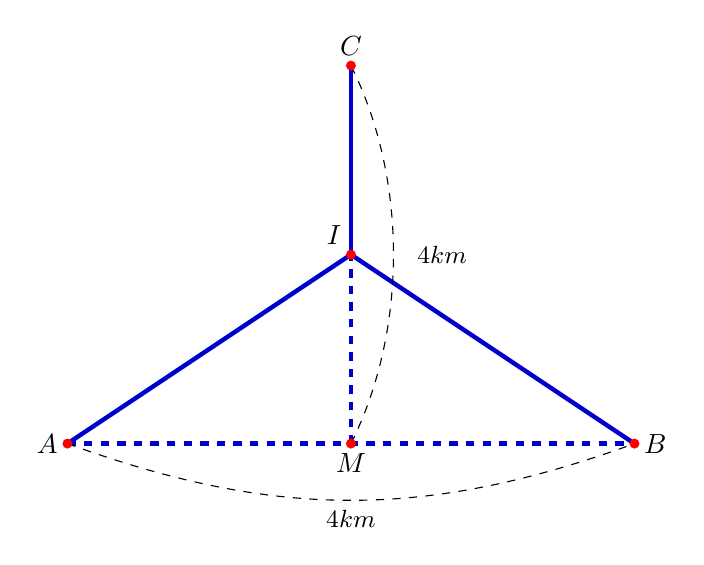
\begin{tikzpicture}[scale=1.2, >=latex]
    % 1. Định nghĩa tọa độ các điểm
    % M làm gốc (0,0), A(-2,0), B(2,0), C(0,4), I(0,1.5)
    \coordinate (M) at (0, 0);
    \coordinate (A) at (-3, 0);
    \coordinate (B) at (3, 0);
    \coordinate (C) at (0, 4);
    \coordinate (I) at (0, 2);

    % 2. Các đường nét đứt
    \draw[dashed,ultra thick, blue!80!black] (A) -- (B); % Đoạn AB
    \draw[dashed,ultra thick, blue!80!black] (M) -- (I); % Đoạn MI

    % 3. Các đường ống chính (nét liền màu xanh)
    \draw[ultra thick, blue!80!black] (C) -- (I); % Đoạn CI
    \draw[ultra thick, blue!80!black] (I) -- (A); % Đoạn IA
    \draw[ultra thick, blue!80!black] (I) -- (B); % Đoạn IB

    % 4. Các cung đường nét đứt đánh dấu kích thước (4km)
    % Cung nét đứt AB bên dưới
    \draw[dashed, black] (A) .. controls (-0.8, -0.8) and (0.8, -0.8) .. (B);
    \node[below, font=\small] at (0, -0.6) {$4\text{km}$};

    % Cung nét đứt MC bên phải
    \draw[dashed, black] (M) .. controls (0.6, 1.2) and (0.6, 2.8) .. (C);
    \node[right, font=\small] at (0.6, 2.0) {$4\text{km}$};

    % 5. Các điểm mốc (chấm đỏ) và nhãn
    \fill[red] (A) circle (1.5pt) node[left, black] {$A$};
    \fill[red] (B) circle (1.5pt) node[right, black] {$B$};
    \fill[red] (C) circle (1.5pt) node[above, black] {$C$};
    \fill[red] (I) circle (1.5pt) node[above left, black] {$I$};
    \fill[red] (M) circle (1.5pt) node[below, black] {$M$};

\end{tikzpicture}
\end{center}
}

\questionShortAnswer{0}{21}{Để chế tác một hạt cường, người ta lấy một khối vật thể có dạng một khối tròn xoay được tạo thành khi quay hình phẳng giới hạn bởi trục Ox và nửa trên của elip  
\(\dfrac{x^2}{1,5^2} + \dfrac{y^2}{1^2} = 1\) (một đơn vị dài trên mỗi trục tọa độ tương ứng với một xăng-ti-mét trong thực tế) quanh trục Ox; sau đó khoan dọc theo trục xoay (xem hình dưới). Lỗ khoan có dạng hình trụ với bán kính \(0,2 \, \text{cm}\) và có trục nằm trên trục xoay. Phần còn lại sau khi khoan là hạt cường, có dạng một khối tròn xoay.  
Thể tích của hạt cường đó bằng bao nhiêu xăng-ti-mét khối (không làm tròn kết quả các phép tính trung gian, chỉ làm tròn kết quả cuối cùng đến hàng phần trăm)?
\begin{figure}[H]
    \centering
    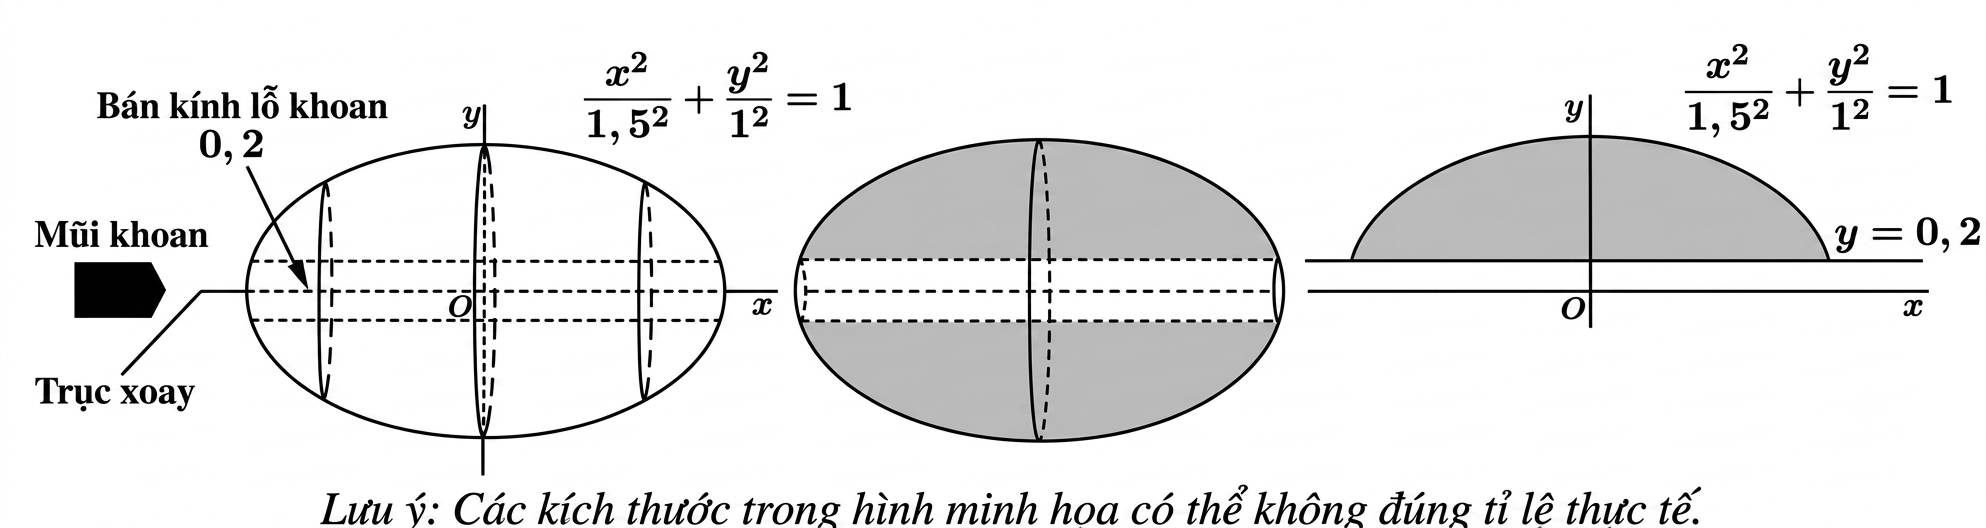
\includegraphics[width=1\textwidth]{images/THPT2026.png}
\end{figure}
}


\questionShortAnswer{0}{22}{Ở một vịnh biển, ngoài khơi xa có một hòn đảo nhỏ. Người ta tiến hành lấn biển để xây dựng khu đô thị và làm một tuyến cáp treo nối khu đô thị với hòn đảo để phát triển du lịch. Xét trong hệ tọa độ \( Oxy \) với đơn vị tương ứng 1km có hòn đảo ở \( O \) thì đường bao của phần đất lấn biển có dạng là một phần của đồ thị hàm số 
\(y = \dfrac{-x^2 + 2}{x}\).
Giả sử tuyến cáp treo được thiết kế nối đảo với đường bao của khu đô thị với độ dài ngắn nhất. Độ dài của tuyến cáp treo là bao nhiêu km (làm tròn kết quả đến hàng phần mười)?
\begin{figure}[H]
    \centering
    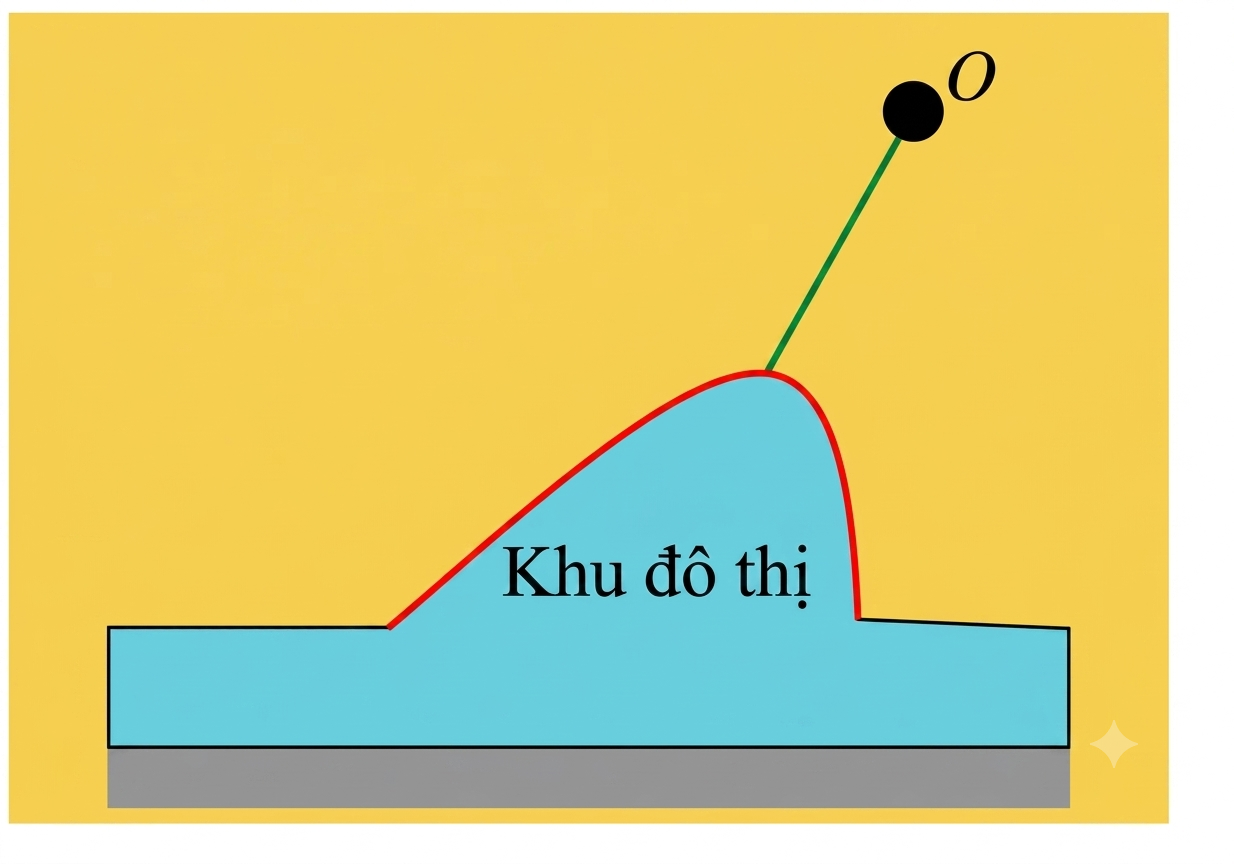
\includegraphics[width=0.4\textwidth]{images/KhuDoThi.png}
\end{figure}
}




\end{document}